%!TEX root = main.tex
\section{Design Guidelines\label{sec:guidelines}}
In this section, we present design guidelines for key components of a visual query system, drawing from our participatory design experience, evaluation study, and literature review in this space. Moreover, we organize our findings in a process model for visual query systems. %Emphasize the fact that the PD process allowed us to identify wh
\subsection{Search-Browse Paradigm}
- What does the act of browsing and searching mean in the context of VQSs
  - browse: viewing ranked result and any recommended results on the side, derived from the data and analysis context.
  - search: act of going from a user's in-the-head concept to an actionable query that could be executed through the VQSs, most work have focussed on sketch, we allow more than this.
  - The challenge of browsing and searching is well-known in information retrieval~\cite{Olston2003}, browse alone is limited by how much a user can browse and process at once, search alone can be ambiguous without sufficient context from looking at example results.
\begin{figure}[h!]
    \centering
    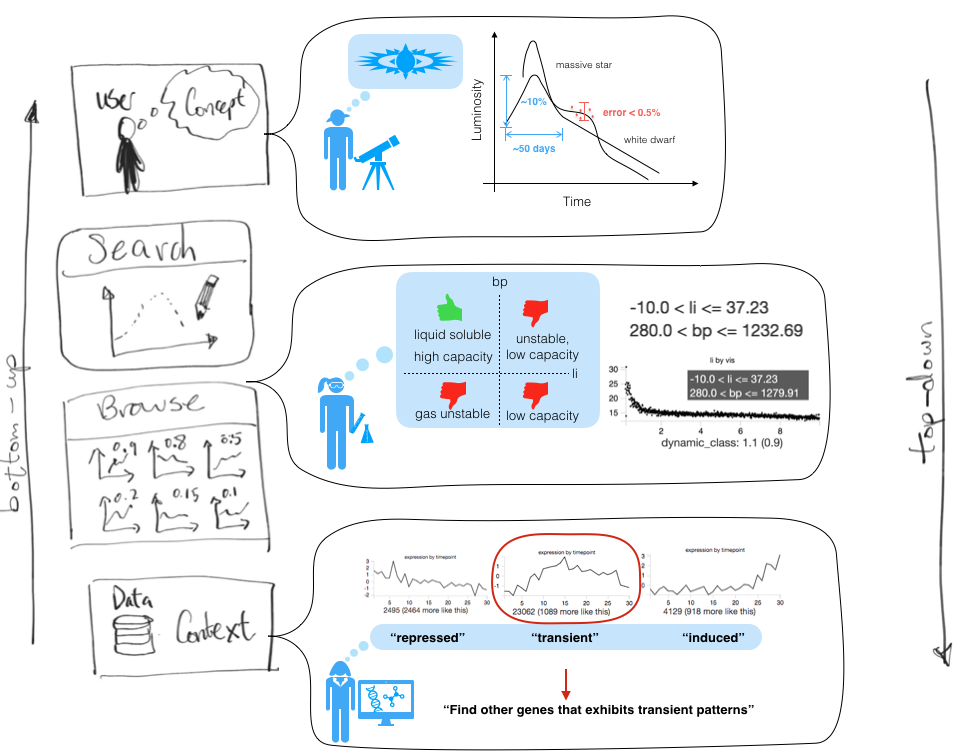
\includegraphics[width=\columnwidth]{figures/search-browse-model.png}
    \vspace{-6pt}\caption{}
    \label{sbmodel}
    \vspace{-5pt}
\end{figure}
\par To contextualize our study results with respect to prior work on how analysts make sense of data, we employ Pirolli and Card's~\cite{Pirolli} information foraging framework for domain-experts. Pirolli and Card's notional model distinguishes between information processing tasks that are \textit{top-down} (from theory to data) and \textit{bottom-up} (from data to theory). Recent work have also used the top-down v.s. bottom-up framework in understanding visualization construction\cite{Mendez2017}. In the context of visualization querying, top-down approaches are query specification based on a user's preconceived notion of what to search for, whereas bottom-up approaches are queries that originate from the data (or equivalently, the visualization).
\par Pirolli and Card's notional model further characterizes the trade-offs between three central activities in the information foraging process: exploring, enriching, and exploiting~\cite{Pirolli}. \textit{Exploring} involves gathering more information during the analysis. \tvcg{In the context of VQSs}, exploring includes viewing representatives and outliers, incidental viewing of other visualizations \tvcg{in the ranked search results}, and querying via drag-and-drop and pattern-loading. \textit{Enriching} involves tasks that narrow down the space of analysis, such as filtering, dynamic class creation, query specification, and querying via input equations and sketching. \textit{Exploiting} involves spending time inspecting the results in more detail, including interpreting each visualization in greater detail or making plotting changes that offer another perspective (smoothing, display, and interpretability settings). We organize the features that we have developed in \zv into these foraging acts, as shown in Figure~\ref{feature_heatmap}.
\par We find that participants often create unexpected workflows that chain together multiple analysis steps, including interactions, controls, and queries in order to address a higher-level research question. We find that participants often construct a central workflow, \tvcg{which they then iterate on while adding additional variations.} Their \emph{central workflow often resembles one of the three foraging acts} that aligns with the type of research question and dataset they are interested in. The variations are based on intermixing their central workflow with the other two foraging \tvcg{acts}.
% We find that participants often have a strong inclination to perform tasks that resembles one of the three foraging act and sparsely intermixed with other activities to support their analysis, depending on the type of research question and dataset they are interested in.
\par As illustrated in Figure \ref{sbmodel}, our search-browse paradigm is motivated by the characteristic challenges and foraging acts each use cases pose on existing VQSs observed in our design study. For example, the genetics participants do not have a preconceived knowledge of what they want to search for in the dataset. They were mostly interested in \textit{exploring} clusters to gain an overall sense what profiles exist in the dataset \tvcg{through representative trends} and therefore queried mainly through drag-and-drop to jumpstart further queries. Point to need for D3 and D4. The variations to their main workflow include changing cluster sizes and display settings to offer them different perspectives on the dataset (\textit{exploit}) and filtering on data attributes (\textit{enriching}).
\par In the astronomy use case, the participants knew the patterns they are looking for, but the patterns are hard to specify and find. The main challenge for the VQS involves finer specification of sketched patterns, such as amplitude and width of the peak and noise level tolerance for defining a pattern match. Describe more in D1. The main workflow for the astronomers in our user study involves \textit{enriching}, either through finer query specification or via filtering data subsets, to increase the probability that their queries would be more accurately matched with what they are looking for.
\par The main workflow for material scientists involves \textit{exploiting}, since they spend the majority of their efforts performing ``close-reading'' of individual visualizations to understand the relationships between physical variables. The participants are able to identify interesting relationships between physical variables when they examine each closely, but they are not sure what patterns to look for to begin with. More in D2.
%For example, G2 knew that there was three repeated measurements that was taken for every timestep, in one of the profiles there was a sharp jump whereas other datapoints are relatively flat, he then concludes by inspecting in the scatterplot view that the rise in gene expression is probably due to an experimental error rather than the activation of a gene, because the other two repeated measurements were similar in magnitude. In other words, the scatterplot view offered him density of points as another proxy to consider that was not offered in the line chart perspective.
 %This is true for both participants with and without a desired pattern in mind. For the participant without a desired pattern (G2), he created groups based on quartile statistics of additional data attributes and recorded the most significant representative pattern.
% [---] out of 9 of our participants had more than one main workflow.
\subsection{Top-down approaches}
  \subsubsection{D1: Increasing Control and Flexibility}
  \subsubsection{D2: Searching with Context}
\subsection{Bottom-up approaches}
  \subsubsection{D3: The Need for Recommendation in VQSs}
  \subsubsection{D4: Closing the loop: query through browsing results}
